\documentclass[12pt, letterpaper]{article}
\usepackage[utf8]{inputenc}
\usepackage{listings}
\usepackage{xcolor}
\usepackage{hyperref}
\usepackage{array}
\usepackage{float}
\usepackage{graphicx}

\graphicspath{ {./images/} }

\definecolor{codegreen}{rgb}{0,0.6,0}
\definecolor{codegray}{rgb}{0.5,0.5,0.5}
\definecolor{codepurple}{rgb}{0.58,0,0.82}
\definecolor{backcolour}{rgb}{0.95,0.95,0.92}
\definecolor{XpathColor}{rgb}{0.0, 0.44, 1.0}

\newcolumntype{M}[1]{>{\centering\arraybackslash}m{#1}}

\lstdefinestyle{mystyle}{
    backgroundcolor=\color{backcolour},   
    commentstyle=\color{codegreen},
    keywordstyle=\color{magenta},
    numberstyle=\tiny\color{codegray},
    stringstyle=\color{codepurple},
    basicstyle=\ttfamily\footnotesize,
    breakatwhitespace=false,         
    breaklines=true,                 
    captionpos=b,                    
    keepspaces=true,                 
    numbers=left,                    
    numbersep=5pt,                  
    showspaces=false,                
    showstringspaces=false,
    showtabs=false,                  
    tabsize=2
}

\hypersetup{
    colorlinks=true,
    linkcolor=blue,
    filecolor=magenta,      
    urlcolor=blue,
    pdftitle={Overleaf Example},
    pdfpagemode=FullScreen,
    }

\setlength{\arrayrulewidth}{0.5mm}
\setlength{\tabcolsep}{15pt}
\renewcommand{\arraystretch}{1.37}

\lstset{style=mystyle}

\title{Ingegneria Dei Dati - Homework 4}
\author{Davide Molitierno - 537969}
\date{16 Novembre 2022}
\begin{document}

\maketitle

\section{Introduzione}
Il seguente progetto ha lo scopo di effettuare l'operazione di \emph{\textbf{"Web Data Extraction"}}, ossia di estrarre informazioni d'interesse su pagine relative allo stesso campo da differenti sorgenti web. Ciascuna caratteristica saliente è stata ottenuta per mezzo di specifiche espressioni \textbf{XPath} e testata successivamente su differenti entità del medesimo tipo.
Nello specifico nella sezione \ref{istruzioni} viene analizzato come sono state individuate le migliori espressioni XPath mentre nelle sezioni \ref{sezione1} e \ref{sezione2} vengono mostrate le informazioni di interesse per i due differenti esercizi e le relative istruzioni utilizzate.
\section{Formato delle istruzioni} \label{istruzioni}
Ciascuna espressione ideata si basa sul medesimo principio per cui, ci si posiziona prima su un elemento invariante il più possibile vicino alla caratteristica di interesse e successivamente ci si muove verso essa. Per tale motivo ciascuna istruzione XPath comincia per un \textbf{"//"} per effetuare la ricerca all'interno dell'intera pagina. Successivamente una parte contenente \textbf{"contains"} o \textbf{"text()="} per posizionarsi in un punto vicino alla caratteristica di interesse che sia presente in ogni pagina relativa a quella tipologia di prodotto. Infine la parte terminale è costituita dal percorso complementare necessario per arrivare all'informazione di interesse. Di seguito viene mostrato un esempio di espressione che utilizza un formato della tipologia sopracitata (l'espressione ricava il titolo dei prodotti della tipologia videogiochi all'interno del sito Amazon.it).

\begin{center}
    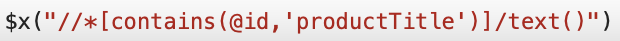
\includegraphics{Espressione XPath}
\end{center}

\section{WDE per videogiochi da Amazon} \label{sezione1}
Tale sezione ha lo scopo di analizzare il lavoro svolto per la realizzazione del primo esercizio richiesto all'interno del progetto, quello di individuare una categoria di prodotti di interesse all'interno del sito web di \href{https://www.amazon.it}{Amazon} ed estrapolare almeno cinque caratteristiche per ciascun prodotto. Per tale esercizio la categoria sulla quale è stato svolto il lavoro è quella relativa ai \href{https://www.amazon.it/s/ref=nb_sb_noss?__mk_it_IT=ÅMÅŽÕÑ&url=search-alias\%3Dvideogames&field-keywords=&crid=2GIVFOZXKUAZD&sprefix=\%2Cvideogames\%2C110}{videogiochi}.  Nello specifico di seguito vengono analizzate le caratteristiche di interesse individuate ed il prodotto su cui sono state ideate e testate le istruzioni XPath che seguono lo schema introdotto nella sezione \ref{istruzioni}.
\subsection{Prodotto tipo e caratteristiche scelte}
Le istruzioni utilizzate sono state ideate sulla base della pagina web di \href{https://www.amazon.it/FIFA-23-Standard-PS4-Italiano/dp/B0B6CKCTXH/ref=sr_1_1?keywords=fifa+23+ps4&qid=1668615637&qu=eyJxc2MiOiIxLjU2IiwicXNhIjoiMC43NSIsInFzcCI6IjAuMzMifQ\%3D\%3D&sprefix=fifa\%2Caps\%2C152&sr=8-1}{Fifa 23} e successivamente sono state testate su diversi altri prodotti simili. Le caratteristiche fondamentali di interesse individuate sono state le seguenti:
 \begin{itemize}
 	    \item Nome;
    \item Prezzo;
    \item Età consigliata;
    \item Lingua;
    \item Data di uscita;
    \item Piattaforma;
    \item Edizione;
    \item Paese di origine.
\end{itemize}
Occorre far notare come alcune di queste caratteristiche non sempre sono presenti per ciascun prodotto. Ad esempio alcune entità non presentano edizioni differenti e per tale motivo la proprietà è assente dal sito mentre per altre Amazon non fornisce alcuna informazione come ad esempio per il paese di origine.
Le istruzioni XPath individuate sono quindi le seguente:
\begin{center}
\begin{table}[!h]
\centering
\begin{tabular}{  |M{3cm} | > {\color{XpathColor}} M{9cm} | }
\hline
\multicolumn{2}{|c|}{\textbf{Espressioni XPath per videogiochi su Amazon}} \\
\hline
 \hline
\textbf{Caratteristica} & \textbf{Espressione XPath} \\[1ex]
 \hline\hline
Nome & \$x("//*[contains(@id,'productTitle')]/text()") \\
Prezzo & \$x("(//*[contains(@id,'corePriceDisplay\_desktop
\_feature\_div')]/div[1]/*/span[1]/text())[1]")  \\
Età consigliata & \$x("//span[contains(text(),'Età consigliata')]/following-sibling::*/text()") \\
Lingua & \$x("//span[contains(text(),'Lingua')]/following-sibling::*/text()") \\
Data d'uscita & \$x("//span[contains(text(),'Data')]/following-sibling::*/text()") \\
Piattaforma & \$x("//*[contains(text(),'Piattaforma:')]/../
text()[2]") \\
Edizione & \$x("//*[text()=' Edizione: ']/*/text()") \\
Paese di origine & \$x("//*[contains(text(),'Paese di origine')]/following-sibling::*/text()") \\
 \hline
\end{tabular}
\end{table}
\end{center}
Infine tali espressioni sono state verificate sui seguenti prodotti: 
\begin{itemize}
	\item \textbf{"God of War"};
	\item \textbf{"Cities Skylines"};
	\item \textbf{"Uncharted 4"};
	\item \textbf{"The Last of Us 2"};
	\item \textbf{"Horizon: Forbidden West"};
	\item \textbf{"Death Stranding"};
	\item \textbf{"Spider-Man Miles Morales"};
	\item \textbf{"Ratchet \& Clank: Rift Apart"};
	\item \textbf{"Gotham Knights"}.
	
\end{itemize}

\section{WDE per piloti di Formula 1}\label{sezione2}
Tale sezione ha lo scopo di analizzare il lavoro svolto per la realizzazione del secondo esercizio del progetto, quello di individuare una entità di interesse e una serie di sorgenti web da cui poter estrarre un insieme di caratteristiche utili per ciascuna entità. Nello specifico l'entità sulla quale è stato svolto il lavoro è quella relativa ai \textbf{piloti di Formula 1}. Le informazioni principali individuate sono state le seguenti:
\begin{itemize}
    \item Team;
    \item Numero;
    \item Data di nascita;
    \item Nazione;
    \item World championships.
\end{itemize}
e in ciascuna sottosezione verrà analizzato come tali informazioni sono state estrapolate per ciascun sito web indicandone il link e l'entità su cui sono state ideate le differenti espressioni. Anche in questo caso, così come fatto per l'esercizio precedente, le espressioni XPath seguono le struttura definita nella sezione \ref{istruzioni}.
\subsection{Formula 1 Official}
\begin{itemize}
	\item Link per il sito web: \href{https://www.formula1.com/en.html}{Formula 1}
	\item Pagina web di riferimento: \href{https://www.formula1.com/en/drivers/lewis-hamilton.html}{Lewis Hamilton}. 
\end{itemize}
\begin{center}
\begin{table}[H]
\begin{tabular}{  |M{3cm} | > {\color{XpathColor}} M{9cm} | }
\hline
\multicolumn{2}{|c|}{\textbf{Espressioni XPath per i piloti di Formula 1 da Formula 1 Official}} \\
\hline
 \hline
\textbf{Caratteristica} & \textbf{Espressione XPath} \\[1ex]
 \hline\hline
Team & \$x("//span[text()='Team']/../following-sibling::*/text() ") \\
Numero & \$x("//*[contains(@class,'driver-number')]/*[1]/text()") \\
Data di nascita & \$x("//span[text()='Date of birth']/../following-sibling::*/text() ") \\
Nazione & \$x("//span[text()='Country']/../following-sibling::*/text() ") \\
World championships & \$x("//span[text()='World Championships']/../following-sibling::*/text() ") \\
 \hline
\end{tabular}
\end{table}
\end{center}
Ciascuna delle seguenti espressioni XPath è stata verificata sulle seguenti entità:
\begin{itemize}
    \item \href{https://www.formula1.com/en/drivers/max-verstappen.html}{Max Verstappen};
    \item \href{https://www.formula1.com/en/drivers/sergio-perez.html}{Sergio Perez};
    \item \href{https://www.formula1.com/en/drivers/george-russell.html}{George Russell};
    \item \href{https://www.formula1.com/en/drivers/fernando-alonso.html}{Fernando Alonso}.
\end{itemize}

\subsection{Al Volante}
\begin{itemize}
	\item Link per il sito web: \href{https://www.alvolante.it}{Al Volante} 
	\item Pagina web di riferimento: \href{https://www.alvolante.it/formula1/piloti/lewis-hamilton}{Lewis Hamilton}. 
\end{itemize}
\begin{center}
\begin{table}[H]
\begin{tabular}{  |M{3cm} | > {\color{XpathColor}} M{9cm} | }
\hline
\multicolumn{2}{|c|}{\textbf{Espressioni XPath per i piloti di Formula 1 da Al Volante}} \\
\hline
 \hline
\textbf{Caratteristica} & \textbf{Espressione XPath} \\[1ex]
 \hline\hline
Team & \$x("//*[contains(@class,'f1-node-car')]/preceding-sibling::*[2]/*/text()") \\
Numero & \$x("//*[text()='Numero di gara']/following-sibling::*/text() ")  \\
Data di nascita & \$x("//*[text()='Data di nascita']/following-sibling::*/text() ") \\
Nazione & \$x("//*[text()='Nazione']/following-sibling::*/text() ") \\
World championships & \$x("//*[text()='Titoli iridati']/following-sibling::*/text() ") \\
 \hline
\end{tabular}
\end{table}
\end{center}

Ciascuna delle seguenti espressioni XPath è stata verificata sulle seguenti entità:
\begin{itemize}
    \item \href{https://www.alvolante.it/formula1/piloti/max-verstappen}{Max Verstappen};
    \item \href{https://www.alvolante.it/formula1/piloti/sergio-perez}{Sergio Perez};
    \item \href{https://www.alvolante.it/formula1/piloti/george-russell}{George Russell};
    \item \href{https://www.alvolante.it/formula1/piloti/fernando-alonso}{Fernando Alonso}.
\end{itemize}

\subsection{Formula1.lne}
\begin{itemize}
	\item Link per il sito web: \href{https://formula1.lne.esl}{Formula1.lne}
	\item Pagina web di riferimento: \href{https://formula1.lne.es/pilotos-f1/lewis-hamilton.html}{Lewis Hamilton}.
\end{itemize} 
\begin{center}
\begin{table}[H]
\begin{tabular}{  |M{3cm} | > {\color{XpathColor}} M{9cm} | }
\hline
\multicolumn{2}{|c|}{\textbf{Espressioni XPath per i piloti di Formula 1 da Formula1.lne}} \\
\hline
 \hline
\textbf{Caratteristica} & \textbf{Espressione XPath} \\[1ex]
 \hline\hline
Team & \$x("//*[contains(@id, 'pilotos\_escuderia')]/h2/*/text()") \\
Numero & \$x("//*[contains(text(), 'N\'{u}mero')]/following-sibling::*/text()")  \\
Data di nascita & \$x("//*[contains(text(), 'Fecha de Nacimiento')]/following-sibling::*/text()") \\
Nazione & \$x("//*[contains(text(), 'Nacionalidad')]/following-sibling::*/text()") \\
World championships & \$x("//*[contains(text(), 'Campeonatos')]/following-sibling::*/text()") \\
 \hline
\end{tabular}
\end{table}
\end{center}

Ciascuna delle seguenti espressioni XPath è stata verificata sulle seguenti entità:
\begin{itemize}
    \item \href{https://formula1.lne.es/pilotos-f1/max-verstappen.html}{Max Verstappen};
    \item \href{https://formula1.lne.es/pilotos-f1/sergio-perez.html}{Sergio Perez};
    \item \href{https://formula1.lne.es/pilotos-f1/george-russell.html}{George Russell};
    \item \href{https://formula1.lne.es/pilotos-f1/fernando-alonso.html}{Fernando Alonso}.
\end{itemize}

\subsection{Motorsport Total}
\begin{itemize}
	\item Link per il sito web: \href{https://www.motorsport-total.com}{Motorsport Total}
	\item Pagina web di riferimento: \href{https://www.motorsport-total.com/formel-1/teams-und-fahrer/fahrer/lewis-hamilton}{Lewis Hamilton}. 
\end{itemize} 
\begin{center}
\begin{table}[H]
\begin{tabular}{  |M{3cm} | > {\color{XpathColor}} M{9cm} | }
\hline
\multicolumn{2}{|c|}{\textbf{Espressioni XPath per i piloti di Formula 1 da Motorsport Total}} \\
\hline
 \hline
\textbf{Caratteristica} & \textbf{Espressione XPath} \\[1ex]
 \hline\hline
Team & \$x("//*[contains(text(), 'Aktuelles Team')]/following-sibling::*/*/text()") \\
Numero & \$x("//*[text()='Startnummer']/following-sibling::*/text()")  \\
Data di nascita & \$x("//*[text()='Geburtsdatum']/following-sibling::*/text()") \\
Nazione & \$x("//*[text()='Nationalität']/following-sibling::*/text()") \\
World championships & N.D. \\
 \hline
\end{tabular}
\end{table}
\end{center}

Ciascuna delle seguenti espressioni XPath è stata verificata sulle seguenti entità:
\begin{itemize}
    \item \href{https://www.motorsport-total.com/formel-1/teams-und-fahrer/fahrer/max-verstappen}{Max Verstappen};
    \item \href{https://www.motorsport-total.com/formel-1/teams-und-fahrer/fahrer/sergio-perez}{Sergio Perez};
    \item \href{https://www.motorsport-total.com/formel-1/teams-und-fahrer/fahrer/george-russell}{George Russell};
    \item \href{https://www.motorsport-total.com/formel-1/teams-und-fahrer/fahrer/fernando-alonso}{Fernando Alonso}.
\end{itemize}
\textbf{Nota:} in questa sorgente web il dato relativo al numero di campionati mondiali vinti non è disponibile e per tale motivo la relativa espressione XPath non è stata riportata.

\subsection{Motor.es}
\begin{itemize}
	\item Link per il sito web: \href{https://www.motor.es}{Motor.es}
	\item Pagina web di riferimento: \href{https://www.motor.es/formula-1/pilotos/lewis-hamilton}{Lewis Hamilton}.
\end{itemize} 
\begin{center}
\begin{table}[H]
\begin{tabular}{  |M{3cm} | > {\color{XpathColor}} M{9cm} | }
\hline
\multicolumn{2}{|c|}{\textbf{Espressioni XPath per i piloti di Formula 1 da Motor.es}} \\
\hline
 \hline
\textbf{Caratteristica} & \textbf{Espressione XPath} \\[1ex]
 \hline\hline
Team & \$x("//*[contains(@class, 'bandera loading')]/following-sibling::*/*[2]/text()") \\
Numero & \$x("//*[contains(text(), 'Dorsal')]/following-sibling::*[1]/text()")  \\
Data di nascita & \$x("//*[contains(text(), 'Fecha de nacimiento')]/following-sibling::*[1]/text()") \\
Nazione & \$x("//*[contains(text(), 'Nacionalidad')]/following-sibling::*[1]/text()") \\
World championships & \$x("//*[contains(text(), 'Campeonatos mundiales')]/following-sibling::*[1]/text()") \\
 \hline
\end{tabular}
\end{table}
\end{center}

Ciascuna delle seguenti espressioni XPath è stata verificata sulle seguenti entità:
\begin{itemize}
    \item \href{https://www.motor.es/formula-1/pilotos/max-verstappen}{Max Verstappen};
    \item \href{https://www.motor.es/formula-1/pilotos/sergio-perez}{Sergio Perez};
    \item \href{https://www.motor.es/formula-1/pilotos/george-russell}{George Russell};
    \item \href{https://www.motor.es/formula-1/pilotos/fernando-alonso}{Fernando Alonso}.
\end{itemize}

\end{document}
